\section{The Latitude Blockchain}\label{sec:design}

In this section, we present a high-level design of the Latitude blockchain. The full-version of this whitepaper shall
contain a very detailed design of each component. We start with an overview of the key design principles that will guide
the rest of the design for the Latitude Blockchain. Its important to note here that for implementation purposes, it
might be possible to use an existing core blockchain for the underlying functionalities and build Latitude as a layer on
top. We shall make these determinations in the full-version of the whitepaper.

\subsection{Design overview}

The purpose of the Latitude blockchain is to become the best platform in the world for decentralized applications for
the Transportation Industry. Specifically, this boils down to constructs in the blockchain that can handle spatial,
mapping, traffic, driving data including data relating to other modalities of transport (bike sharing, walking, even air
routes later on). Figure \ref{fig:lat-arch} presents the architecture of the Latitude blockchain in terms of the core
technological innovations that will be built into it.

\begin{figure}[t]
    \centering
    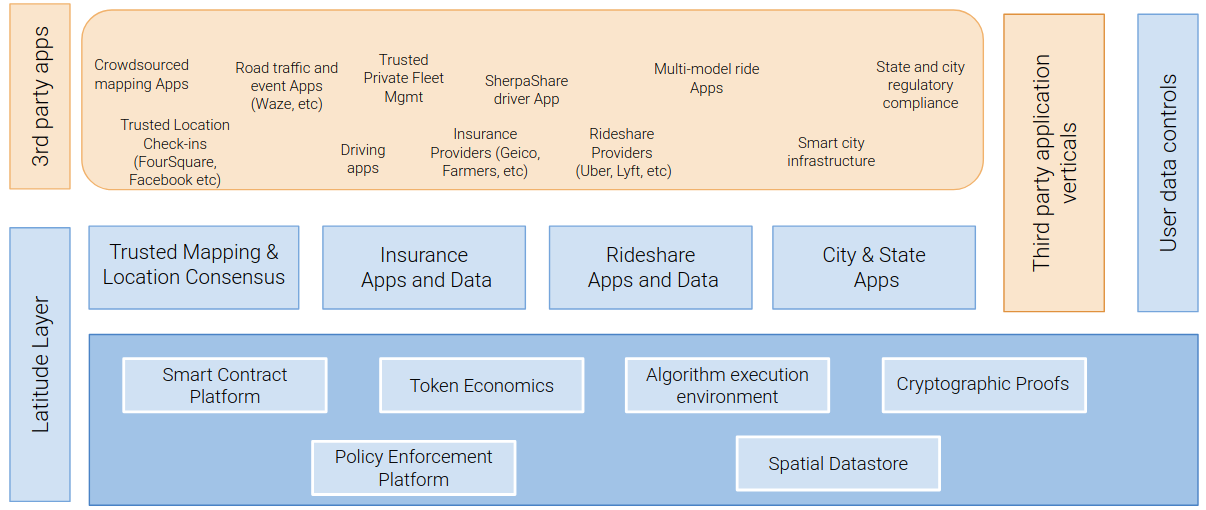
\includegraphics[width=1.00\textwidth]{latarch.png}
  \caption{Architecture of the Latitude Blockchain and associated platform ecosystem.}
    \label{fig:lat-arch}
\end{figure}

\subsection{Spatial datastore}
One of the central aspects of the Latitude blockchain is a geo-spatial datastore that fundamentally understands various
datatypes that are specific to transportation data. This datastore can use existing GIS databases that allow
de-centralized storage and access. The types of data include (i) georaphic data such as location (latitude, longitude),
(ii) mapping data such as roads, terrain, addresses, etc, (iii) sensor data such as driving data, driver score, miles
driven, route information, etc, (iv) multi-modal transport data such as biking, walking and other means of transport.
Each of these data types have very special characteristics which the underlying datastore can be optimized for and allow
for programming using what we call the {\em Latitude Smart Contract} framework. 

The datastore would include spatial, quad-tree or an R-tree based indexes for efficient querying and other operations that
most Geographic Information Systems (GIS) would support in a centralized manner today. It would also include functions
to compute heatmaps, driving maps and statistics such as Traffic predictions including real-time analytics. Depending on
how Latitude evolves, the datastore can include additional functionalities to support the data sharing among autonomous
vehicles since they use most of the similar datatypes mentioned above. The datastore would support circular, rectangular
and other range queries, K-nearest neighbor searches, route optimization algorithms, etc. Figure
\ref{fig:geo_spatial_query} shows some of the queries that such a datastore can support.

\begin{figure}[t]
    \centering
    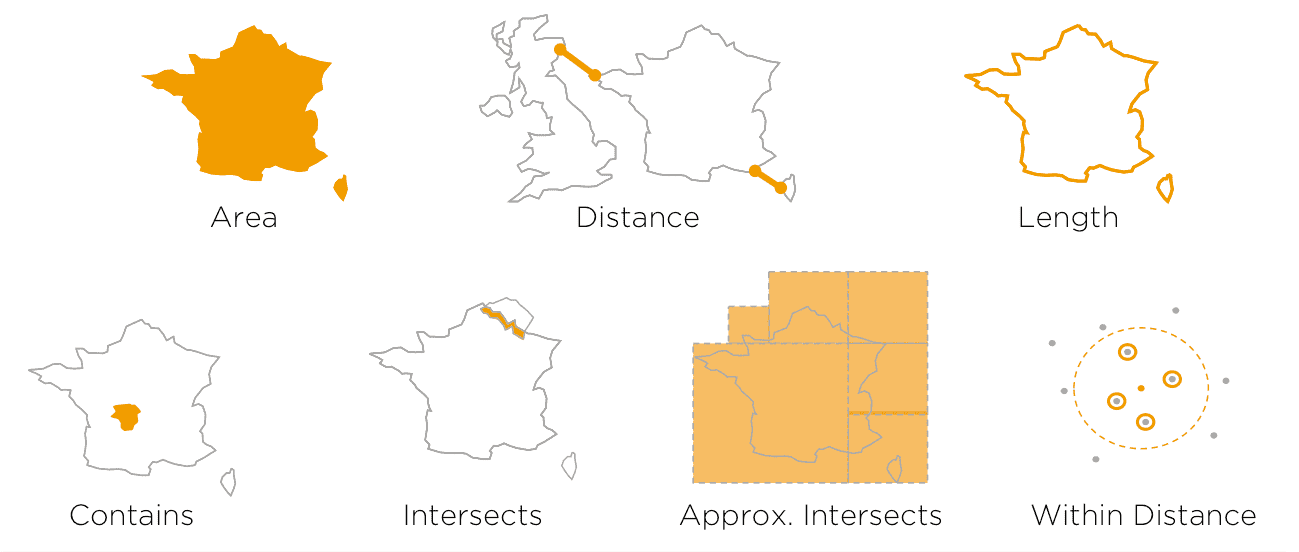
\includegraphics[width=0.70\textwidth]{geospatial_query.png}
  \caption{Examples of Geo-spatial queries that a spatial datastructure can support on the Latitude blockchain.}
    \label{fig:geo_spatial_query}
\end{figure}


%Datastore
% - Optimized for Geographic, Geo-spatial data.
% - Location, Mapping data and computation.
% - Ability to Store, index, query and build smart contracts optimized for such data.
% - Support for various spatial indexes.
% - Location heatmaps.
% - Indexing road and driving data.
% - Primitives for storing driving data for autonomous vehicles

\subsection{Cryptographic primitives}

Latitude makes use of strong cryptographic protocols, primitives, encryptions, secure hash function, certificates,
multi-party key distribution, proxy key reencryption, Elliptic-curve based Digital Signatures \cite{ecdsa} and other
state-of-the-art mechanisms to provide strong security, privacy, access control, confidentiality and anonymity
guarantees. Specifically for geo-spatial data such as location, anonymity guarantees can be very important part of data
sharing smart contracts and privacy policies such as GDPR \cite{gdpr}. Latitude provides anonymity guarantees using
cryptographic set preserving computations as derived from research in \cite{kissner_set}. These can be suitably modified
to allow for location-based anonymity which requires stronger guarantees when compared to set-based anonymity methods
\cite{divanis_kanon,xu_loc_anon}.

Latitude also uses Merkle trees for cryptographic proof of audit, existence of data, verifiable computations and such
\cite{becker2008}. These proof can be shared as certificates among participants or be used in the Latitude smart
contract system discussed later. The proofs allow for verification such as if a certain amount of data was shared, or as
simple as if a certain data exists. They also allow for the maintenance of a cryptographic log of all operations that
happen on the network. These techniques are similar to the ones used by some of the other blockchains today
\cite{buterin_merkle}.


%Cryptographic primitives for:
% - Security and privacy of data.
% - Anonymity guarantees using cryptographic set operations.
% - Enforcement of privacy when sharing data.
% - Sharing of “computation” instead of data when possible.
% - For eg: Sharing of DriverScore using a vetted algorithm.
% - Sharing proximity to a landmark instead of lat/lng.
% - Ability to find bad actors.
% - Detect privacy, anonymity and security violations.
%
%Cryptographic proofs for applications:
% - Proof of Location. 
% - Proof of ride. 
% - Proof of mapping 
%      (road/landmark exists or does not exist).
% - Proof of driver score 
% - Open, trusted, understood driver score computation algorithms.
% - Cryptographic proofs can be shared among entities, safely, securely.


In addition to these standard primitives discussed above, Latitude provides a host of other proofs that are tailor made
for geo-spatial, mapping, location and sensor data for driving. Thes proofs that can be used by applications, users and
other participants in the network. The network can be extended to create new forms of proofs as the application needs
grow. The proofs include the ones listed below but are not limited to these:

 \begin{itemize}
     \item Proof of location: This is perhaps the most easily motivated functionality that the Latitude blockchain can
         provide. Proof of location is a cryptographic credential that proves that a given user, entity or participant
         is physically present at a given location or a relative location to another participant. The proof of location
         has been explored by other blockchains such as Platin \cite{platin}. Latitude shall provide the mobile, browser
         and sensor SDKs that can directly tie into the datastore to provide consensus based proofs. These proofs can
         unlock applications such as access to facilities or help increase trust in crowdsourced mapping, traffic and incident
         reports.
     \item Proof of ride: Provides a proof that a particular user has taken a ride from point A to point B using a
         certain type of transport. This proof can be used across multi-modal ride platforms such as bike or car rides.
         This can be later extended to include bus trips, flights, train rides and so on. The proof of ride is also
         built using the same mobile SDK which can gather trust on the nature and parameters of the ride.
     \item Proof of landmark (mapping): This proves the existence of a particular landmark, such as a monument, a
         building, a sign post at a given lat/lng. This can also be used to prove the existence of a particular road or
         the lack of. These proofs can be constructed using the proof of location and added consensus among users and
         can form the backbone for verified mapping and landmark data.
     \item Proof of driver score: This proof can be computed on the blockchain over the data aggregated on the
         datastore. The algorithm itself shall be made available to the nodes either as an executable docker image or an
         opensource version. This allows different nodes to run the computation and create a certificate of a certain
         driver score which can then be attributed to the driver or user. This open framework can also allow different
         driver score algorithms to co-exist in the system creating a community where better driver score algorithms can
         be agreed upon and used as the industry standard.
     \item Proof of traffic:  Similar to the driver score, traffic is also an algorithm that looks at the statistics of
         location and speed data on roads. The proof is similarly computed through consensus and recorded as a
         certificate on the blockchain. The proof could be about real-time traffic or historic traffic patterns which
         can be shared with smart city applications or census or regulatory bodies.
     \item Proof of routes: Similar to the functionality in the popular Waze app, this is about whether there exists a
         certain route (or a better route) from point A to point B. More the consensus higher the trust and for example,
         if a user actually makes that route from A to B, that helps create the proof of its existence. This is useful
         for trusted and verifiable mapping / routing applications.
 \end{itemize}
\subsection{Latitude Smart contract system}

\begin{figure}[t]
    \centering
    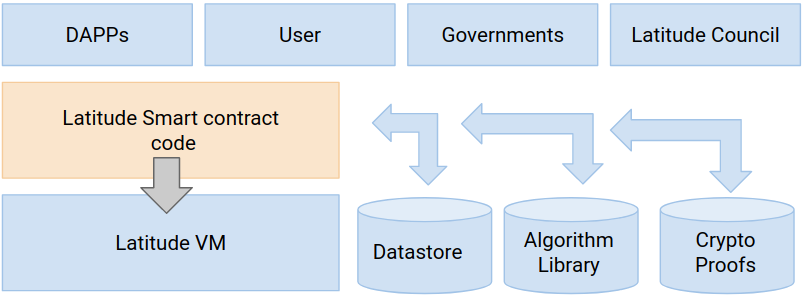
\includegraphics[width=0.60\textwidth]{lat_sc.png}
  \caption{Architecture of the Latitude Smart Contract framework.}
    \label{fig:lat-sc}
\end{figure}

Smart contracts are self-executing contracts with the terms of the agreement between various participants on the
blockchain. For the Latitude blockchain, this can be the user, a regulatory body or an application written by an
insurance company or the city. The contract is directly written into lines of code in a certain language. Popular smart
contract frameworks today include ones used by Ethereum which runs on the Ethereum Virtual Machine (EVM), the Neo which
runs on the NeoVM and the EOS blockchain which runs on the WASM (WebAssembly VM).

The smart contract code and the agreements contained therein exist across the distributed, decentralized Latitude
blockchain network.  Because of this, Smart contracts permit trusted transactions and agreements to be carried out among
disparate, anonymous parties without the need for a central authority, legal system, or external enforcement mechanism.
They render transactions traceable, transparent, and irreversible as the state is always available on the Latitude
blockchain.

Figure \ref{fig:lat-sc} shows the high-level architecture of the Latitude Smart contract system. Latitude uses a
modified version of Solidity (or the new Vyper programming language) as used by the Ethereum Virtual Machine. The choice
of this language is based on the production quality of the EVM, the language tools available in the community for
creating contract code, developer support and talent pool. Latitude shall add enhancements to the language to support
new spatial data types, indexes, cryptographic proofs and other mechanisms that are fundamental to the platform. Some of
the goals of the smart contract system include the ability to convert data policies such as GDPR \cite{gdpr} into
Latitude smart contract code which can then get automatically verified and enforced on the blockchain.  Also its
possible to share location data in an emphemeral manner for a specific purpose -- the data item gets automatically
destroyed using consensus and smart contract constructs on the blockchain. An example includes a user sharing their
location with an app for a very small duration of time.

As showsn in Figure \ref{fig:lat-sc}, the smart contract code has access to the datastore, cryptographic proofs
(including algorithms to create proofs), an algorithm library (which hosts algorithms such as traffic, driver score
etc). These are directly accessible through language constructs making it easy to write high quality smart contract
code. The smart contract execution framework and related functionalities are accessible to dapps, entities such as
users, governments and the Latitude Council (discussed later in the Governance section) on the system. 

The Latitude smart contract system can becomes the world's first such smart contract framework specifically tailored for
transportation data and applications.

% Smart contract system for Transportation
% applications.  - Ability to convert “policies” such as GDPR into smart contract code.  - Example, self destruct data
% after a time period.  - Sandboxed trusted execution environment: - For algorithms: - DriverScore, Location heatmaps,
% Statistics.  - Enforcing or verifying privacy and other govt policies/regulations.


\noindent
\subsection{Cryptoeconomics and Governance}

Crytpeconomics and governance refer to the incentive structure in the Latitude blockchain and the decentralized decision
making structure. These discussions go hand-in-hand as they specify how the blockchain functions in a distributed and
decentralized manner in the real world.

\subsubsection{Crytpoeconomics}
Crytoeconomics refers to the mechanics of the protocol underlying the blockchain operations which creates incentives
for the various stakeholders. For example, in the Latitude Blockchain it is possible to reward users for sharing their data
for certain purposes. For example, users can be rewarded if they share traffic data or accident information or better
routes. This is similar to the Waze model but creates legitimate rewards for users that have meaningful value outside
the Waze application. For an overview of cryptoeconomics in the blockchain space, please see \cite{sinclair_crypto}.

The core building block of the cryptoeconomics in Latitude is the Latitude Token, or LAT. This will be transacted in
each and every micro-transaction that takes place on the blockchain to create the right incentives, enforce smart
contracts and penalize Byzantine behavior. One of the fundamental design principles behind the protocol for the LAT
token is to create incentives assuming nodes are greedy and are interested in maximizing their gain. We will also build
safeguards against reasonable amount of collusion among nodes to subvert the system. The design is crafted such that the
best way for a node to maximize its revenue would be to participate with full honesty.

Latitude shall employ a Proof of Stake model (delegated or non-delegted) for particpation and core node-level mining. This mechanism has recently
gained popularity among a notable number of blockchains \cite{dpos_steemit}. This also allows for deposit slashing as a
technique to tackle Byzantine behavior. Latitude will employ techniques such as Minimal Slashing \cite{buterin_slashing}
for Byzantine fault tolerance and safety under distributed asynchronous operation.

\subsubsection{Governance}
Governance refers to a decentralized manner in which decisions are made using a consensus mechanism on the blockchain.
Decisions include basic constructs whether a node can join or leave the network. Or it can include key decisions on
whether an upgrade should be mandated on every node, a given participant such as a data provider should be penalized. It
could also include issues where humans get involved, such as when a user complains of a loss of privacy or a breach in
contract.

Recently blockchains have been moving towards governance using a small set of participants, such as trusted miners in
the case of Stellar and Ripple \cite{stellar_gateway}. The EOS blockchain uses a similar concept of a core set of block
producers who are elected based on a nomination and voting process \cite{eos_producers}. For discussion around
Governance in Ethereum, refer to \cite{buterin_gov}. Latitude uses a similar concept of a {\em council} of participants.
These are entities (nodes or organizations) that have demonstrated participating using earned trust through honest
operation, accumulating stake, demonstrated good intent and establishing trust. Some members of this council might
include the core Latitude developers which allows them to implement operations such as updates, bug fixes and so on. The
council members shall be elected using the an election protocol on the blockchain. It might be possible to directly
nominate certain council members such as regulatory bodies who have general interest in user rights, privacy and
enforcement. 

 - Crypto-incentives for honest operation.
 - Penalties for malicious intent.
 - Governance based on consensus and roles using a council.
 - Council members elected using voting, stake and established trust.
 - Some council members can have restricted access.
 - Eg: US govt can have voting rights on US data/users, etc.

\subsubsection{User incentives}
Token economics allow for the creation of what we call user incentives. These are protocol constructs in the blockchain
that allow users to benefit from the value they create for the ecosystem. Refer to \cite{token_ecos} for an overview on
incentive mechanisms to reward users for various methods of participation in the network. In general, the Latitude token
ecosystem will be based on market economics, that is, supply and demand from various participants will be the primary
driver for prices and incentives in the network. This philosophy falls in line with decentralized control and operation
while also allowing for creating most reward for honest behavior in the network.

The ability of user incentives to exist in a decentralized manner can be disruptive to existing incumbents in the
sharing economy space, such as Uber, Lyft, Airbnb, etc since users can get rewarded in a tangible manner for their
contributions \cite{sharing_eco_bc}. Consumers shifted to apps in the sharing economy as they provided cheaper and
better alternatives to traditional services like Uber and Airbnb. However, since all transactions go through these
centralized providers, the platform owners determine the fees, percentages and are in complete control of any data
practices and policies which cannot be verified. They often become accused of predatory behavior. Using blockchain based
incentives, sharing and open-source software these problems can be addressed in a singular fashion.

As an exmaple, consider the Ridesharing application. As users contribute data on what rides they are taking, it becomes
possible for the network to reward them with tokens. They could, upon sufficient contribution, redeem them for free
rides or share with them others on the network. A similar model can be adopted for data concerning driver behavior where
drivers using different apps and sensor algorithms can elect to share their data towards building a better driver score
in return for suitable incentives.

User incentives:
 - Users have full control over their data and computation.
 - Users can issue or request proofs to carry over to other applications.
 - User’s have incentive to share data, participate in improving the common denominator.
 - Malicious intent, Byzantine behavior.
   - Can be detected using a combination of consensus and incentives.
   - Best interest of users to act honestly by design.

\noindent
\subsection{Performance considerations}

When thinking of performance, one of the key metrics that is hotly debated in the community is transactions per second.
Bitcoin is know for its long time to produce a block, on the order of minutes which limits the number of transactions
the network can process. Figure \ref{fig:tps_speed} shows a comparison of the major blockchains today with respect to
this cricial metric. Note that these blockchains shown in the Figure are primarily evaluated against the concept of a
transaction which represents a transfer of assets, goods or monetary value digitally on the blockchain. Stellar and
Ripple are two blockchains that have gained popularity for financial transactions as they tout a higher transcation
velocity. 

\begin{figure}[t]
    \centering
    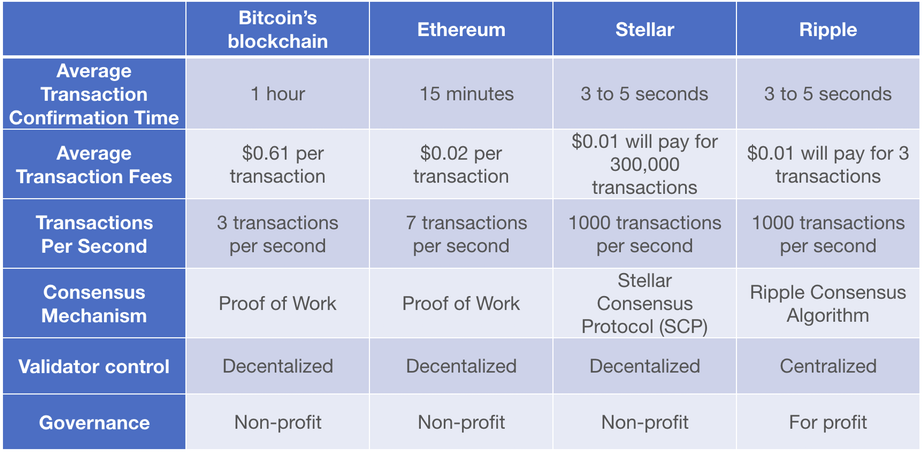
\includegraphics[width=0.90\textwidth]{tps_speed2.png}
  \caption{Comparison of transactions per second of the major blockchains today.}
    \label{fig:tps_speed}
\end{figure}

In the context of Latitude, the performance of the blockchain is important. The blockchain will handle different types
of data and transactions which will require different levels of consensus and trust. Figure \cite{fig:tps_lat} shows the
different types of transactions that the Latitude blockchain can process and the performance we expect to achieve. Shown
are four types of transactions:
\begin{itemize}
    \item Datastore transactions: These refer to basic transactions to store data values into the geo-spatial data
        store. For instance, if a user shares their driving data, this can include the sensor information, lat/lng of
        the trip taken and any mapping data collected. For ridesharing applications, this can include any multi-model
        ride details that the user has booked. We expect the blockchain to be able to process close to 1-10 million
        transactions per second, since most such transactions require very low level of consensus and can tolerate 
        eventual consistency \cite{eventual_con}.
    \item Algorithmic computations: These refer to transactions which include executing known algorithms on the
        blockchain. For instance, this could include the computation of various driver behavior algorithms with the
        computation being shared among certain participants on the network. Another computation could include statistics
        such as real-time traffic or aggregate traffic statistics shared with a city for better zoning and planning
        purposes. The amount of consensus required is relativel small but higher than datastore operations in order to
        ensure correct execution of algorithms and lack of malicious intent. Also such operations would require strong
        consistency for their CRUD funtionalities. We expect the Latitude design to support 10-100K transactions per
        second at its peak usage.
    \item Data sharing contracts: These transactions refer to the creation, deletion or arbitration of long-term sharing
        smart contracts between participating entities. For instance, it could include a new contract between an
        insurance company and a data provider for sharing certaint types of driver score data for certain geographic
        locations. Since these transactions have higher value they require larger amount of trust and consensus in the
        system. Latitude shall support a transaction speed of around 100-1000 transactions per second for this category.
    \item Governance operations: The Governance operations require the highest amount of trust and full consensus of the
        network. These include voting to add/remove council members, critical council decisions such as forks or
        updates/upgrades, decisions on high-value smart contract disputes, etc. The transaction velocity is low for
        reasons of trust, accuracy and correctness and thus we expect the Latitude blockchain to support 1-10
        transactions per second under this category.

\end{itemize}

Another metric of importance for Latitude is the storage capacity in the network. This can be important for
datastore operations. We expect the storage capacity, network bandwidth and any other computing resource to become
available on an incentived model as determined by usage contracts. For instance, if a user is willing to share data with
a data consumer, the consumer should be able to allocate token resources to provision the network with sufficient
storage. The token can be used to purchase storage using other blockchain storage providers such as Filecoin, Siacoin or
Golem can be used to incentivize nodes to directly supplant on-chain storage.

\begin{figure}[t]
    \centering
    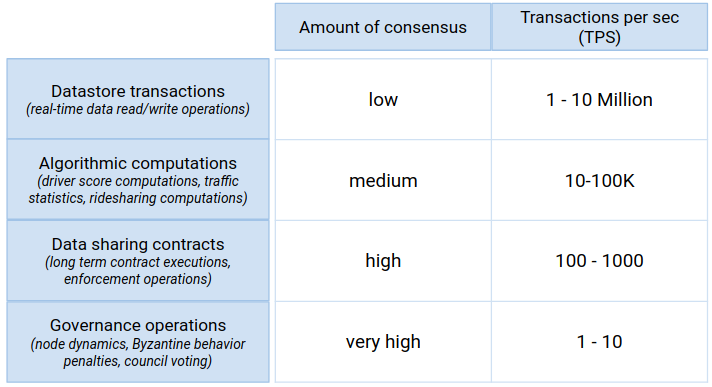
\includegraphics[width=0.75\textwidth]{tps_lat2.png}
  \caption{Expected Transaction per second velocity of various types of functionalities on the Latitude Blockchain.}
    \label{fig:tps_lat}
\end{figure}

